\begin{center}
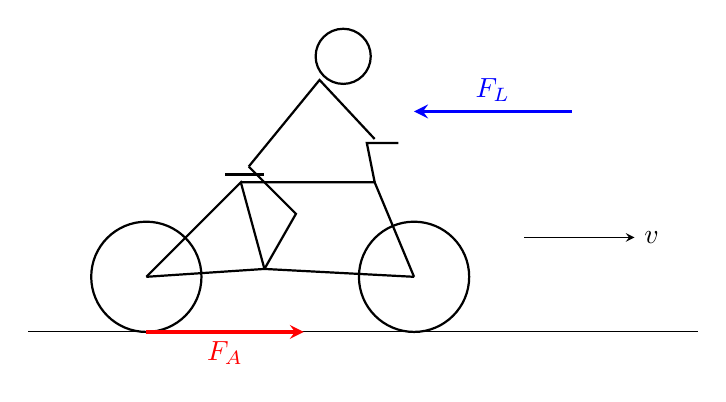
\begin{tikzpicture}[>=stealth]
 \draw (-0.5,0) -- (8,0);
 \draw[thick] (1,0.7) circle (0.7);
 \draw[thick] (4.4,0.7) circle (0.7);
 \draw[thick] (1,0.7) -- (2.5,0.8) -- (4.4,0.7);
 \draw[thick] (1,0.7) -- (2.2,1.9) -- (2.5,0.8);
 \draw[thick] (2.2,1.9) -- (3.9,1.9) -- (4.4,0.7);
 \draw[thick] (3.9,1.9) -- (3.8,2.4) -- (4.2,2.4);
 \draw[thick] (2.0,2.0) -- (2.5,2.0);
 \draw[thick] (2.3,2.1) -- (3.2,3.2) -- (3.9,2.45);
 \draw[thick] (2.3,2.1) -- (2.9,1.5) -- (2.5,0.8);
 \draw[thick] (3.5,3.5) circle (0.35);
 \draw[->, very thick, red] (1,0) -- (3,0);
 \node[red, below] at (2,0) {$F_\text{A}$};
 \draw[->, very thick, blue] (6.4,2.8) -- (4.4,2.8);
 \node[blue, above] at (5.4,2.8) {$F_\text{L}$};
 \draw[->] (5.8,1.2) -- (7.2,1.2) node[right] {$v$};
\end{tikzpicture}
\end{center}

Die Geschwindigkeit ist konstant, also ist die resultierende Kraft auf das System „Fahrrad + Sie“ null (Trägheitsgesetz). In Fahrtrichtung muss deshalb eine gleich grosse Kraft wirken wie der Luftwiderstand nach hinten (die Rollreibung ist hier vernachlässigt):
\begin{align}
 F_\text{A} &= F_\text{L} = \result{\FAnP{0}{2}}
\end{align}

Die Kräfte zwischen Füssen, Pedalen, Kette und Hinterrad sind innere Kräfte des Systems. Von aussen greift die Antriebskraft an der \emph{Berührungsstelle zwischen Hinterrad und Strasse} an: Das Hinterrad stösst die Strasse nach hinten, und die Strasse stösst das Hinterrad als Reaktion (Haftreibungskraft) nach vorne.
